
\documentclass[11pt,a4paper,computermodern]{article}


\usepackage[
%	includeheadfoot,
	width=172mm,
	top=18mm,
	bottom=18mm,
	bindingoffset=4mm
	]{geometry}



%%% Typeface packages
\usepackage[utf8]{inputenc}
\usepackage[T1]{fontenc}
\usepackage{fontawesome}

\usepackage{multirow}
\usepackage{tabularx}
\usepackage{booktabs}
\usepackage[flushleft]{threeparttable}

%%% Graphics packages
\usepackage{graphicx}
\usepackage{subcaption}


%%

\usepackage[
	sorting=none,
	backend=bibtex,
	style=nature,
	url=false,        
	doi=false,         
	isbn=false,
	minbibnames=1,  
	maxbibnames=10
]{biblatex}

\usepackage{hyperref}
\hypersetup{
	colorlinks=false,
	hidelinks=true,
}

%%
%\newcommand{\code}[1]{\colorbox{light-gray}{\texttt{#1}}}
\newcommand{\code}{\texttt}

%%
\title{A Proposal for Spotify Data Governance}
\date{}


\begin{document}

\maketitle

\vspace{-10mm}

Spotify, founded in 2006 and now serving over 450 million users globally, including 200 million premium subscribers, is the world’s leading audio streaming platform. Operating in 180+ countries, Spotify relies heavily on data to deliver personalized experiences, power its recommendation engine, and drive content and marketing strategies. The company manages a vast and complex data ecosystem that includes user behavioral data (e.g., listening habits, search history), content metadata (e.g., song attributes, podcast tags), subscription and billing data, advertising engagement metrics, and localized market insights. This rich data landscape is foundational to Spotify’s innovation but also demands a robust governance framework to ensure data quality, compliance with global privacy regulations like GDPR and CCPA, and secure, ethical use of user information.


\section{Spotify's Data Landscape}

\subsection*{Data Maturity Assessment}

Spotify must adapt its data governance to the constraints imposed by its rapid growth. The company can be considered between level 3 and 4 on Gartner's data maturity scale We provide in this section a comprehensive assessment of its maturity for each of the knowledge areas of the DAMA-DMBoK data management framework.

\begin{figure}[ht]
	\begin{subfigure}[h]{0.4\linewidth}
		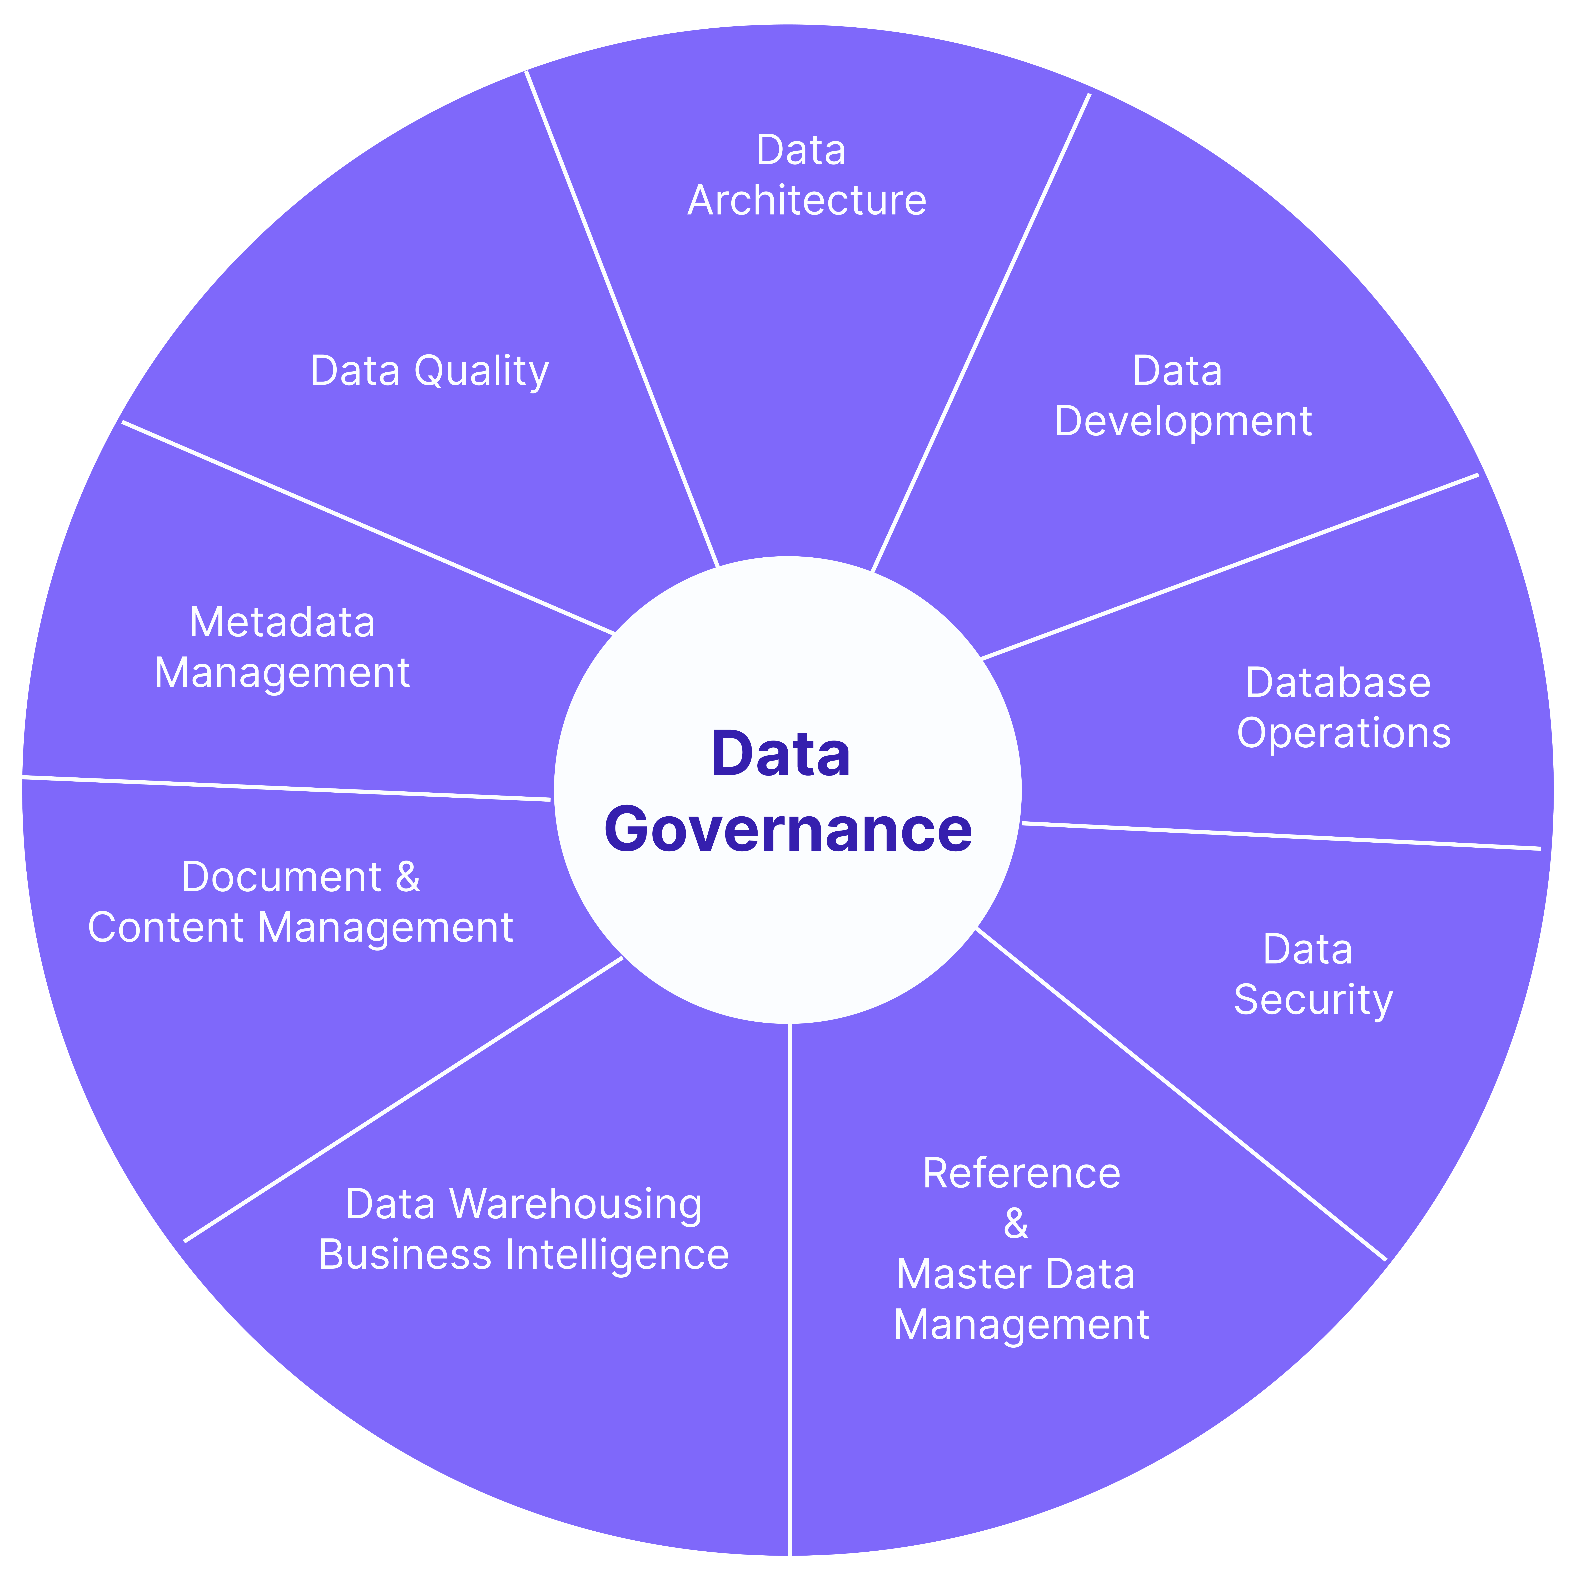
\includegraphics[width=\linewidth]{./figures/DMBoK_v3}
	\end{subfigure}
	\hfill
	\begin{subfigure}[h]{0.58\linewidth}
		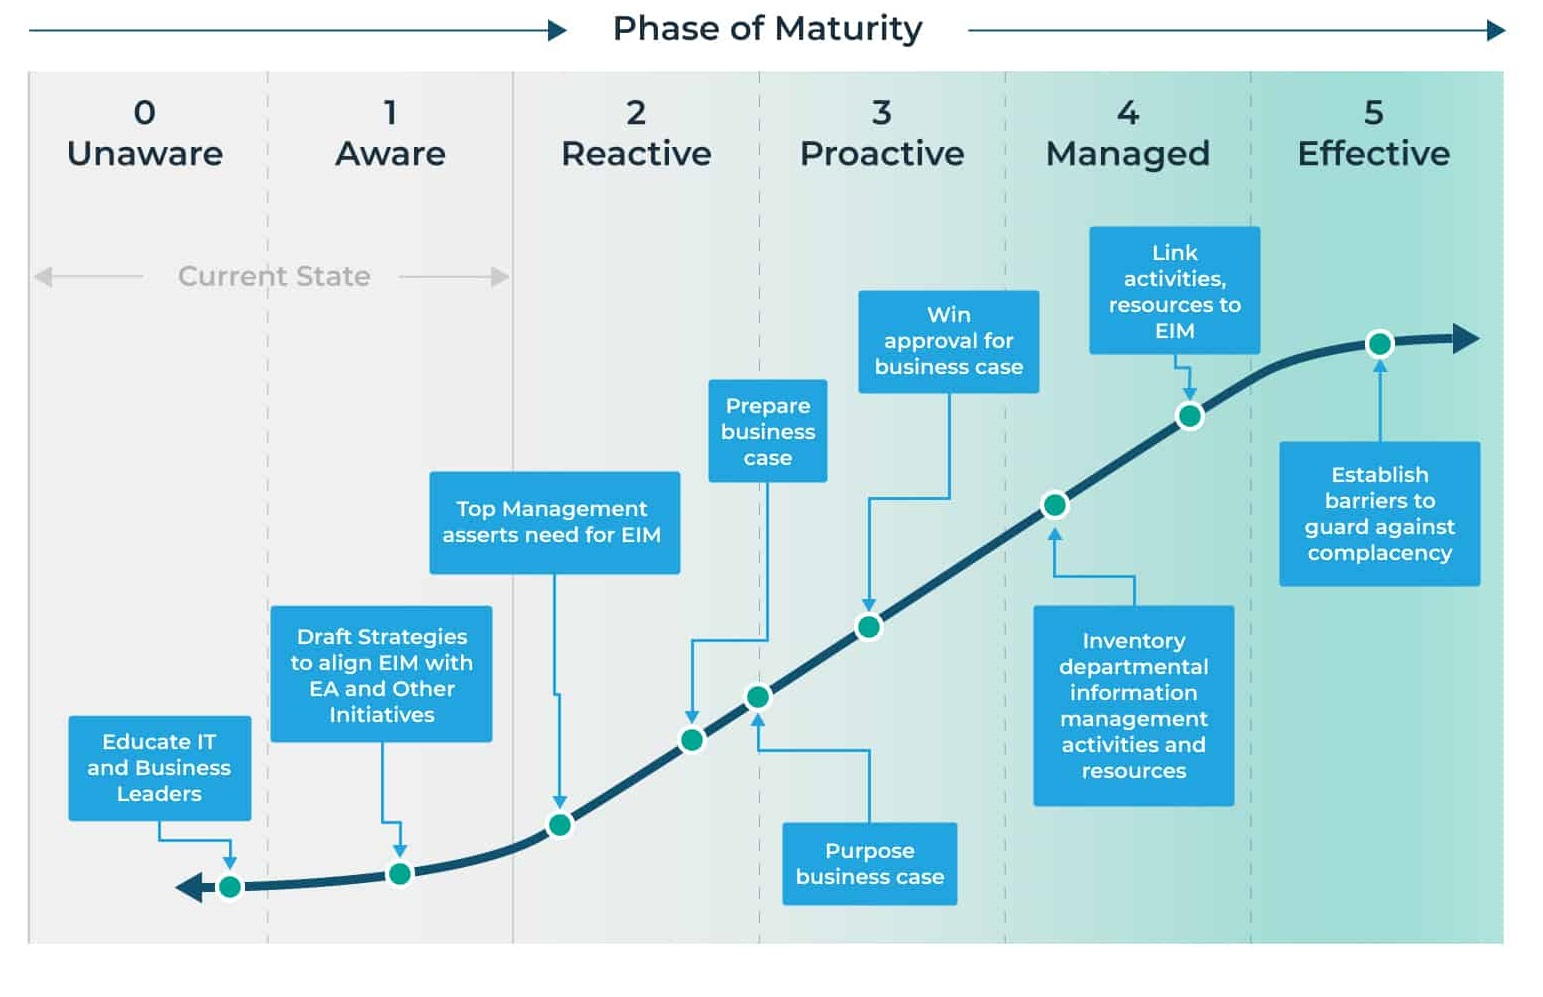
\includegraphics[width=\linewidth]{./figures/data_maturity}
	\end{subfigure}
%	%\caption{Proposed OLTP database structure.}
	\label{fig:DataManagement}
\end{figure}

\begin{itemize}
	\item \textbf{Data Governance: level 2 - Reactive}\\
	No unified governance framework exists; data ownership and stewardship are informal and siloed.
	\item \textbf{Data Architecture: level 3 - Proactive}\\
	Sophisticated architecture using cloud, lakes, and databases, but lacks enterprise-wide integration and standardization.
	\item \textbf{Data Development: level 3 - Proactive}\\
	Strong ML and engineering capabilities, but development practices are fragmented with inconsistent documentation.
	\item \textbf{Data Operations Management: level 3 - Proactive}\\
	Real-time data pipelines are robust, but operational monitoring and SLAs are inconsistent across teams.
	\item \textbf{Data Security Management: level 4 - Managed}\\
	Advanced controls are in place, but evolving regulatory environments create ongoing compliance risks.
	\item \textbf{Reference and Master Data Management: level 2 - Reactive}\\
	Artist, content, and user master data are inconsistently managed across departments, leading to duplication.
	\item \textbf{Data Warehousing and Business Intelligence Management: level 3 - Proactive}\\
	Analytics infrastructure is powerful but suffers from limited cross-team visibility and fragmented key performance indicators.
	\item \textbf{Document and Content Management: level 2 - Reactive}\\
	No centralized taxonomy or governance for podcast metadata, contracts, or localized content documentation.
	\item \textbf{Meta-data Management: level 2 - Reactive}\\
	Inconsistent metadata practices and lack of a centralized data catalog hinder discoverability and quality.
	\item \textbf{Data Quality Management: level 2 - Reactive}\\
	Data quality is reactive; missing validation processes and automated cleansing across data pipelines.
	\item \textbf{Data Compliance: level 3 - Proactive}\\
	Active GDPR/CCPA efforts, but no unified compliance framework; needs structured oversight and audits.
	\item \textbf{Data Literacy: level 2 - Reactive}\\
	Data usage varies by team; limited formal training and a strong reliance on technical staff for interpretation.
\end{itemize}


\subsection*{Key Governance Challenges}

Spotify's growth and innovation depend on turning its advanced data infrastructure into a well-governed, integrated, and trusted data ecosystem. This will require formalizing data governance policies, building roles like Data Stewards, and establishing foundational practices in metadata, quality, and literacy — all while maintaining compliance in a complex global regulatory environment.

\begin{itemize}
	\item \textbf{Data silos and frangmentation}\\
	Independent data handling by departments like marketing, product, and engineering leads to inconsistent, incomplete data views and hinders unified analytics.
	\item \textbf{Regulatory Compliance Complexity}\\
	Navigating diverse regulations (GDPR, CCPA) across more than 180 countries requires a dynamic compliance strategy and stronger oversight.
	\item \textbf{Low metadata quality and standards}\\
	Metadata is inconsistently applied, and data quality issues negatively impact core systems like the recommendation engine.
	\item \textbf{Access and integration barriers}\\
	Disconnected systems delay innovation and product launches; employees lack timely access to needed data.
	\item \textbf{User privacy and trust}\\
	Increasing user awareness of data rights demands greater transparency, consent management, and anonymization protocols.
	\item \textbf{Weak data culture}\\
	While data is critical to strategy, there is limited enterprise-wide literacy, governance awareness, or data stewardship.
\end{itemize}



\section{Spotify's Data Governance Framework}

In this section we provide a unified approach to managing data across all functions, regions, and systems. This policy applies to all data collected, stored, processed, or shared by Spotify globally, and all Spotify teams, including engineering, marketing, content, legal, and product.


\subsection*{Data Governance Principles}

Accountability: Clear data ownership and stewardship across all datasets.
Transparency: Documented metadata, data lineage, and access logs.
Compliance: All data practices must meet international and local regulatory standards.
Integrity: Ensure accuracy, completeness, and reliability of all business-critical data.
Security: Protect data confidentiality, availability, and integrity at every lifecycle stage.
Collaboration: Encourage cross-functional sharing and integration of data.


\subsection*{GDPR and CCPA Compliance}




\subsection*{Roles and Responsibilities}

\begin{table}[ht]
	\centering
	\begin{threeparttable}
		\caption{Roles and Responsibilities summary table.}
		\label{table:roles}
		\begin{tabularx}{0.99\textwidth}{c >{\centering\arraybackslash}X}
			\toprule
			Role & Key Responsibilities  \\
			\midrule
			Chief Data Officer (CDO) & Leads data governance strategy, policies, and KPIs. \\
			Data Protection Officer & Ensures compliance with GDPR/CCPA, handles breaches, DSARs. \\
			Data Stewards & Manage data definitions, quality, and metadata. \\
			Head of Engineering & Builds systems to support secure, governed data access. \\
			Legal Counsel & Advises on compliance risks and regulatory interpretation. \\
			Product \& Marketing Leads & Ensure responsible use of user data and accurate analytics. \\
			\bottomrule
		\end{tabularx}
	\end{threeparttable}
\end{table}



\section{Implementation of the Data Governance Framework}

\subsection*{Organizational Model}

Given the size of the company and the amount of data to manage, the recommended approach is that of the center of excellence (CoE) model. In this model, a central data governance team, lead by the CDO, defines the standards and practices for data management. It also provides training and support to the data teams embedded in each department (e.g. marketing, product, engineering). A cross-functional governance committee of data engineers, legal councils, data protection officer and business leaders oversights data management and compliance.

In the context of this organizational model, both full-code and low/no-code solutions will be used.
\begin{itemize}
	\item \textbf{Full-code} technologies are mandatory among the CoE team. They must also be available among the embedded teams to allow for interfacing data manipulation with the CoE team.
	\item \textbf{Low/No-code} technologies are key to the embedded teams in the different department. They provide high data availability for a large volume of non-tech people such as business analysts.
\end{itemize}


\subsection*{Technologies and tools}

\begin{table}[ht]
	\centering
	\begin{threeparttable}
		\caption{Recommended technology tools to support Spotify's data governance framework.}
		\label{table:tools}
		\begin{tabularx}{0.99\textwidth}{c >{\centering\arraybackslash}X >{\centering\arraybackslash}X}
			\toprule
			Category & Purpose & Examples \\
			\midrule
			Data cataloging & Central metadata management, data discovery & \href{https://www.alation.com/}{Alation}, \href{https://atlas.apache.org/}{Apache Atlas}, \href{https://atlan.com/}{Atlan}, \href{https://www.collibra.com/}{Collibra} \\
			Data quality & Automate data profiling, validation, alerts & \href{https://www.ataccama.com/}{Ataccama}, \href{https://www.informatica.com/products/data-quality.html}{Informatica Data Quality}, \href{https://www.soda.io/}{Soda}, \href{https://www.talend.com/products/data-integrity-governance/}{Talend} \\
			Compliance monitoring & Manage user consent, automate data subject access requests (DSARs) & \href{https://bigid.com/}{BigID}, \href{https://www.onetrust.com/}{OneTrust}, \href{https://trustarc.com/}{TrustArc}, \href{https://verasafe.com/}{VeraSafe} \\
			Data security & Protection of sensitive user and payment data & \href{https://www.dataguard.com/}{DataGuard}, \href{https://www.splunk.com/}{Splunk}, \href{https://cpl.thalesgroup.com/encryption/vormetric-data-security-platform}{Vormetric} \\
			Lineage and integration & Track data flow across systems & \href{https://atlas.apache.org/}{Apache Atlas}, \href{https://www.informatica.com/products/data-quality.html}{Informatica} \\
			\bottomrule
		\end{tabularx}
	\end{threeparttable}
\end{table}

It is of course recommended to avoid redundancy by selecting a single tool for a given purpose.


\subsection*{Pilot implementation}

Spotify will begin with a pilot implementation in the user data domain. The steps are:
\begin{itemize}
	\item[1] Select Stakeholders: CDO, Data Stewards (Marketing, Product), DPO, Legal.
	\item[2] Audit Existing Data: Identify sources, access logs, quality gaps.
	\item[3] Apply Governance Rules: Define metadata, access controls, validation checks.
	\item[4] Configure Tools: Deploy data catalog and privacy software for pilot scope.
	\item[5] Train Teams: Deliver sessions on new policies, roles, and tools.
	\item[6] Monitor Metrics: \% of high-quality user records, of DSARs handled on time, user trust/engagement metrics
	\item[7] Review \& Iterate: Adjust processes before scaling to other domains.
\end{itemize}

The pilot implementation will have the following target performance indicators:
\begin{itemize}
	\item 90\% service-level agreement compliance on data subject requests
	\item 80\% data literacy training adoption in pilot teams
	\item  less than 3\% data quality error rate in governed domains
\end{itemize}


\end{document}